\pdfminorversion=7
\documentclass[14pt]{beamer}

\usepackage[utf8]{inputenc}
\usepackage[english]{babel}
\usepackage[T1]{fontenc}
\usepackage{newtxmath}
% \usepackage[
% bibstyle=authoryear, % alphabetical
% citestyle=authoryear, % alphabetical
% backend=biber,
% maxnames=2,
% maxbibnames=99]{biblatex}
% \addbibresource{literature.bib}
% \AtBeginBibliography{\tiny}
% \SetCiteCommand{\parencite}
\usepackage{graphicx}
\usepackage{xcolor}
\usepackage{url}
\usepackage{pifont}
\usepackage{booktabs}
\usepackage{amsmath}
\usepackage{mathtools}
\usepackage{bbm}
\usepackage[mathcal]{euscript}
\usepackage{geometry}
\usepackage{listings}
\usepackage{cancel}

\beamertemplatenavigationsymbolsempty
\setbeamerfont{page number in head/foot}{size=\large}
\setbeamertemplate{footline}{%
\hfill%
\usebeamercolor[fg]{page number in head/foot}%
slide
\usebeamerfont{page number in head/foot}%
\insertframenumber%
\kern2pt\vskip1pt%
}

\definecolor{backcolor}{rgb}{0.2,0.2,0.2}
\definecolor{keycolor}{rgb}{0.8,0.471,0.196}
\definecolor{codecolor}{rgb}{0.9,0.9,0.9}
\definecolor{stringcolor}{rgb}{0.416,0.718,0.349}
\definecolor{commentcolor}{rgb}{0.5,0.5,0.5}
\lstdefinestyle{pythonstyle}{
    backgroundcolor=\color{backcolor},
    keywordstyle=\color{keycolor},
    commentstyle=\color{commentcolor},
    %numberstyle=\tiny\color{codegray},
    stringstyle=\color{stringcolor},
    basicstyle=\ttfamily\scriptsize\color{codecolor},
    breakatwhitespace=false,
    breaklines=true,
    captionpos=b,
    keepspaces=true,
    showspaces=false,
    showstringspaces=false,
    showtabs=false
}

\lstset{style=pythonstyle}

\begin{document}

\begin{frame}[plain,noframenumbering]
\begin{center}
{\usebeamercolor[fg]{title}\usebeamerfont{title}Transformations in Three Dimensions\par}
\vfill

\setbeamercolor{boxcolor}{bg=blue!5}
\begin{beamercolorbox}[sep=0.5em,center]{boxcolor}
\textbf{Alexander Fabisch}\\
DFKI GmbH, Robotics Innovation Center
\end{beamercolorbox}

\vfill
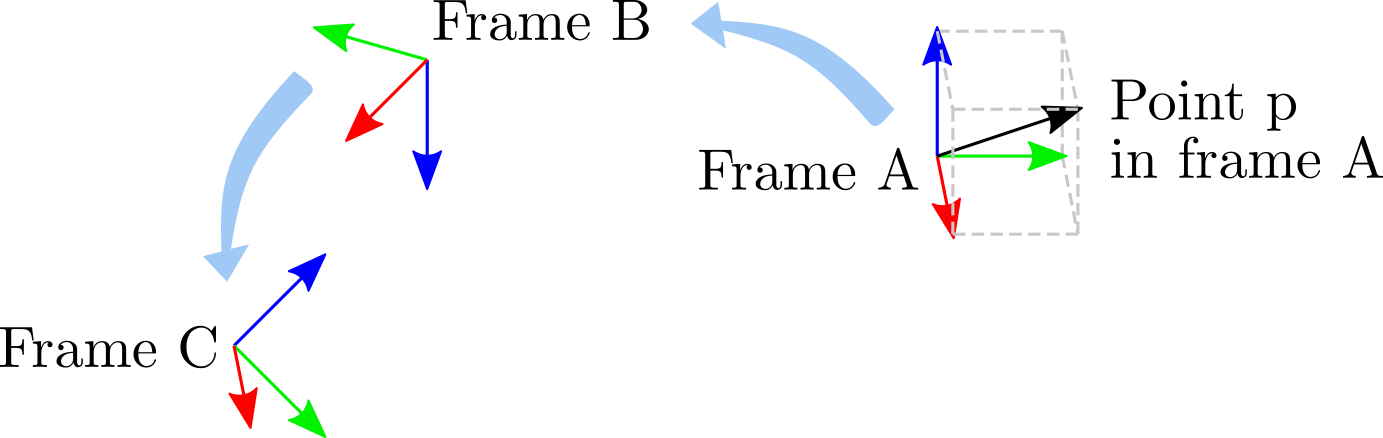
\includegraphics[width=\textwidth]{images/transformation_modeling}
\vfill
\url{https://github.com/dfki-ric/pytransform3d}
\end{center}
\end{frame}

\begin{frame}{Features of pytransform3d}
\begin{itemize}
\item operations for most common representations of rotation / orientation and
  translation / position
\item conversions between those representations
\item clear documentation of conventions
\item tight coupling with matplotlib to quickly visualize (or animate)
  transformations
\item the TransformManager which organizes complex chains of transformations
\item the UrdfTransformManager which is able to load transformations from URDF
  files
\item a matplotlib-like interface to Open3D’s visualizer to display geometries and
  transformations
\end{itemize}
\end{frame}

\begin{frame}
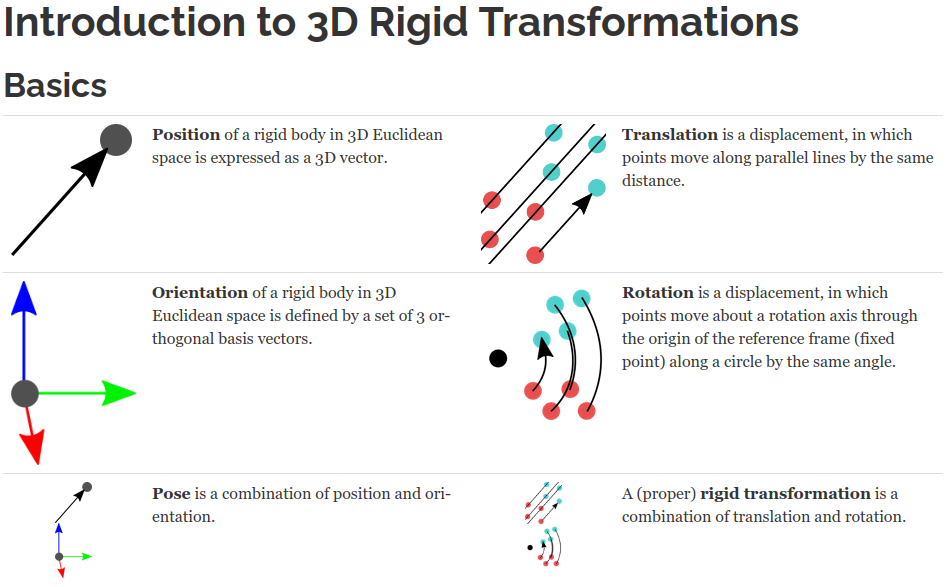
\includegraphics[width=\textwidth]{images/introduction}
\end{frame}

\begin{frame}{Frames}
A \textit{coordinate reference} \textbf{frame} in 3D Euclidean space is defined by an origin (position) and 3 orthogonal basis vectors (orientation) and it is attached to a rigid body.

\vfill

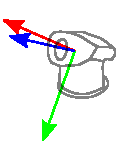
\includegraphics[height=1.9cm]{images/conventions_camera}
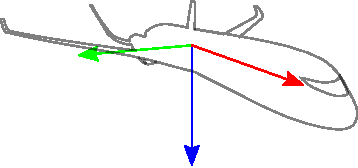
\includegraphics[height=1.9cm]{images/conventions_plane}
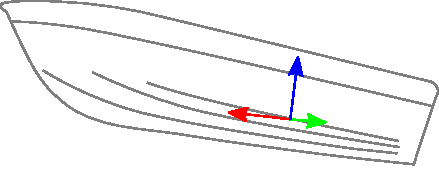
\includegraphics[height=1.9cm]{images/conventions_ship}

\vfill

\setbeamercolor{boxcolor}{bg=blue!10}
\begin{beamercolorbox}[wd=\textwidth,sep=1em]{boxcolor}
We will use RGB lines to indicate basis vectors.
\end{beamercolorbox}
\end{frame}

\begin{frame}[fragile]{Imitation Learning}
\begin{columns}
\begin{column}{0.4\textwidth}
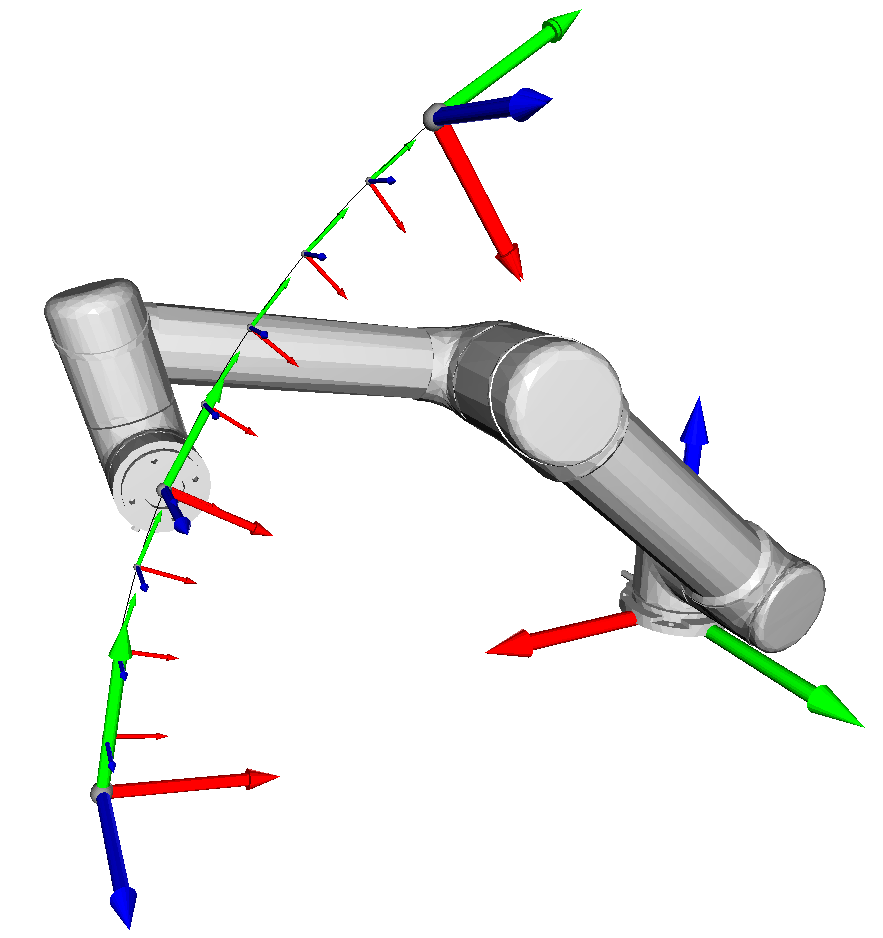
\includegraphics[width=\textwidth]{images/movement_primitives_cart_dmp_ur5}
\end{column}
\begin{column}{0.6\textwidth}
\begin{itemize}
\item Given: one or more demonstrated solutions to a problem (trajectory)
\item How can we represent it?
\item Movement primitives:
\url{https://github.com/dfki-ric/movement_primitives}
\end{itemize}
\end{column}
\end{columns}
\end{frame}

\begin{frame}{SO(3) (SO: special orthogonal group)}
--- group of all rotations in 3D

--- represented by 3D rotation matrices

\vfill

\begin{center}
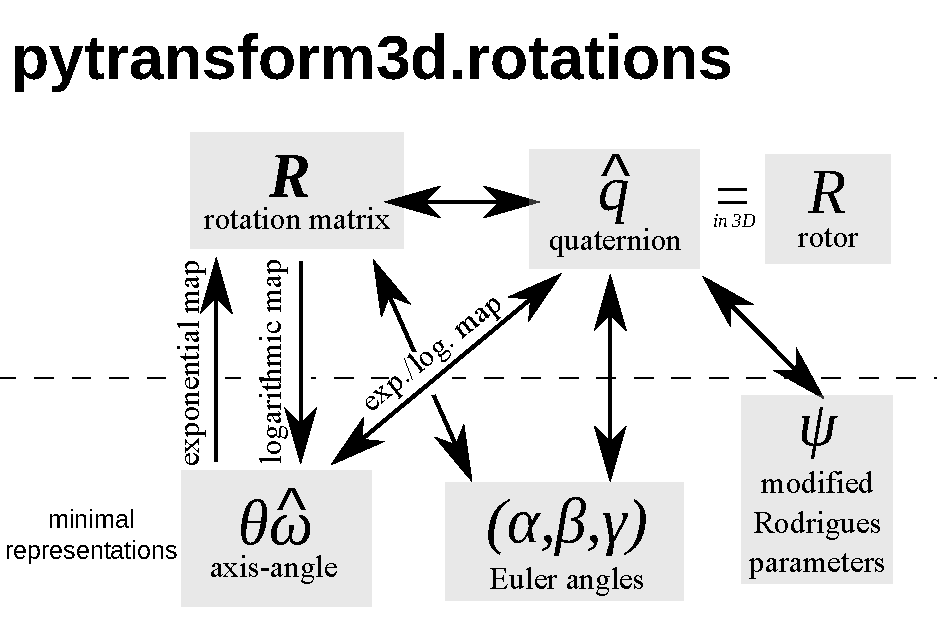
\includegraphics[width=9cm]{images/rotations}
\end{center}
\end{frame}

\begin{frame}[fragile]{Imitation Learning}
\begin{columns}
\begin{column}{0.4\textwidth}
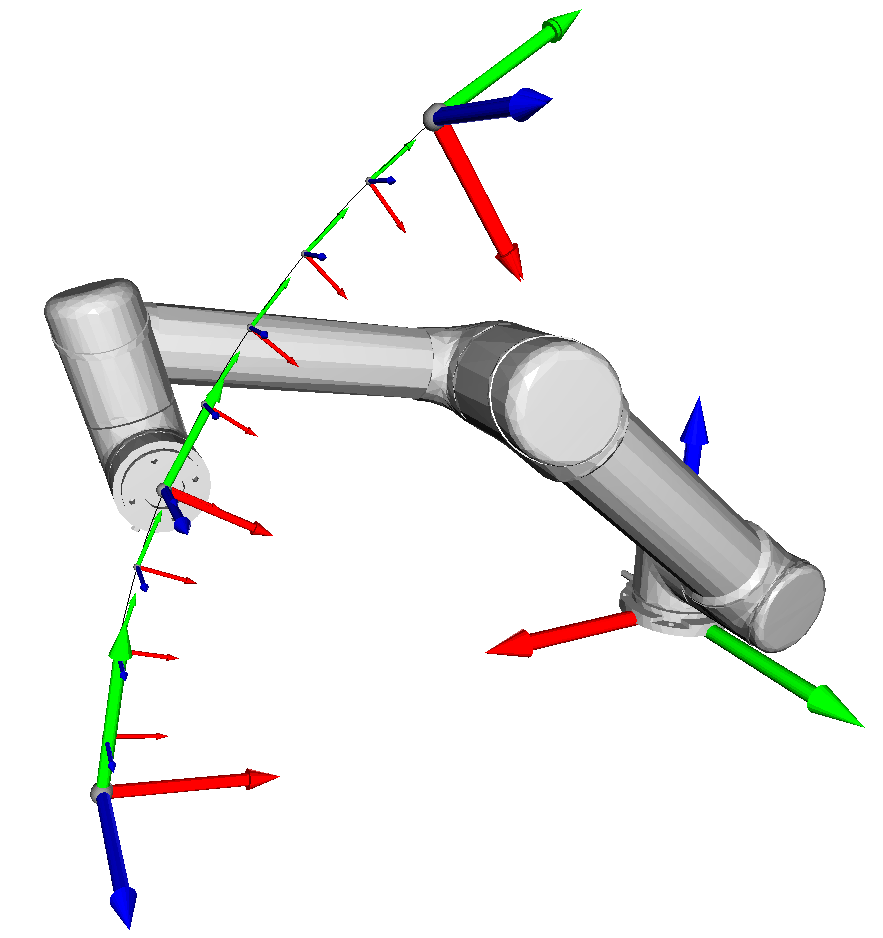
\includegraphics[width=\textwidth]{images/movement_primitives_cart_dmp_ur5}
\end{column}
\begin{column}{0.6\textwidth}
Common problems
\begin{itemize}
\item Rotation matrices have 6 constraints that are not easy to enforce
\item Minimal representations $\in \mathbb{R}^3$ have singularities
\item Quaternions $q \in \mathbb{S}^3$ have an ambiguity: $q = -q$
\begin{lstlisting}[language=Python]
from pytransform3d.rotations import pick_closest_quaternion
q1 = pick_closest_quaternion(
    q1, q2)
\end{lstlisting}
\end{itemize}
\end{column}
\end{columns}
\end{frame}

\begin{frame}[fragile]{Visualizer}
\begin{columns}
\begin{column}{0.4\textwidth}
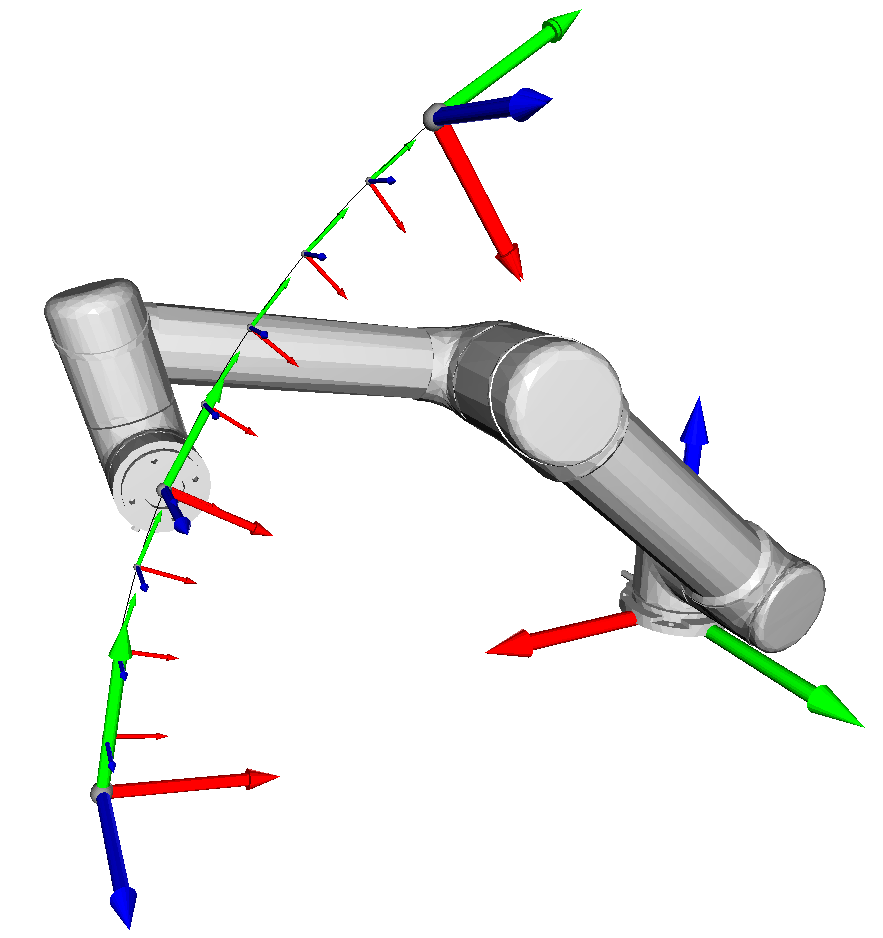
\includegraphics[width=\textwidth]{images/movement_primitives_cart_dmp_ur5}
\end{column}
\begin{column}{0.6\textwidth}
\begin{lstlisting}[language=Python]
import pytransform3d.visualizer as pv


fig = pv.figure()
fig.plot_transform(s=0.3)

fig.plot_graph(
    urdf_transform_manager,
    "ur5_base_link",
    show_collision_objects=True,
    show_frames=True)

fig.plot_transform(ee2base_start)
fig.plot_transform(ee2base_end)

pv.Trajectory(trajectory
    ).add_artist(fig)

fig.view_init()
fig.show()
\end{lstlisting}
\end{column}
\end{columns}
\end{frame}

\begin{frame}[fragile]{Concatenation of Uncertain Transforms}
\begin{center}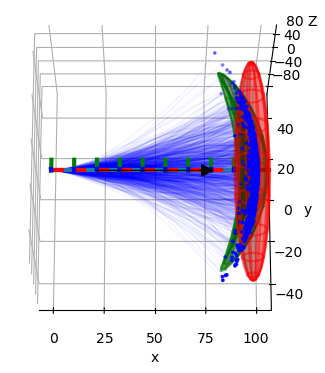
\includegraphics[width=0.4\textwidth]{images/state_estimation}\end{center}
\vskip -0.4cm
\begin{itemize}
\item Uncertainty of angular velocity about z-axis
\item \textcolor{blue}{Blue}: Monte Carlo sampling of trajectories
\item \textcolor{red}{Red}: Gaussian of MC-sampled final positions
\item \textcolor{green}{Green}: Propagated uncertainty in \textit{exponential coordinates}
(\textbf{banana distribution})
\end{itemize}
\end{frame}

\begin{frame}{SE(3) (SE: special Euclidean group)}
--- group of all proper rigid transformations in 3D

--- represented by transformation matrices

\vfill

\begin{center}
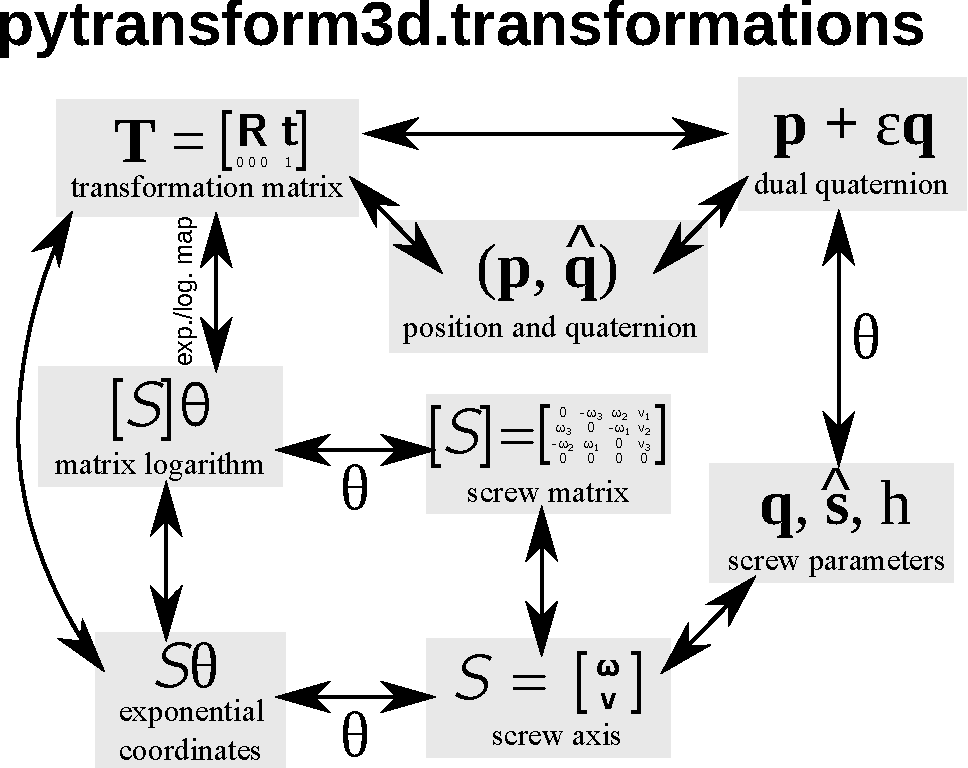
\includegraphics[width=7cm]{images/transformations}
\end{center}
\end{frame}

\begin{frame}{Transformation Matrices}
\[
SE(3) = \biggl\{ \boldsymbol{T} = \left(
\begin{array}{cc}
\boldsymbol{R} & \boldsymbol{t}\\
\boldsymbol{0} & 1
\end{array}
\right) \in \mathbb{R}^{4 \times 4}
| \boldsymbol{R} \in SO(3), \boldsymbol{t} \in \mathbb{R}^3 \biggr\}
\]

\[
\boldsymbol T =
\left( \begin{array}{cc}
    \boldsymbol R & \boldsymbol t\\
    \boldsymbol 0 & 1\\
\end{array} \right)
=
\left(
\begin{matrix}
r_{11} & r_{12} & r_{13} & t_1\\
r_{21} & r_{22} & r_{23} & t_2\\
r_{31} & r_{32} & r_{33} & t_3\\
0 & 0 & 0 & 1\\
\end{matrix}
\right)
\]
\end{frame}

\begin{frame}{Exponential Coordinates}
\setbeamercolor{boxcolor}{bg=blue!10}
\begin{beamercolorbox}[wd=\textwidth,sep=1em]{boxcolor}
Screw axis: $\left[ \begin{array}{c}\hat{\boldsymbol{s}} \\ \boldsymbol{q} \times \hat{\boldsymbol{s}} + h \hat{\boldsymbol{s}}\end{array} \right] = \textcolor{red}{\mathcal{S}} \in \mathbb{R}^6$
\end{beamercolorbox}

\vfill

\hfill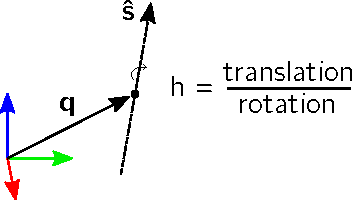
\includegraphics{images/screw_axis}

\vfill

\begin{beamercolorbox}[wd=\textwidth,sep=1em]{boxcolor}
Exponential map: $Exp(\textcolor{red}{\mathcal{S}\theta}) = \boldsymbol{T} =
\left( \begin{array}{cc}
\boldsymbol R & \boldsymbol t\\
\boldsymbol 0 & 1\\
\end{array} \right)
\in SO(3)$
\end{beamercolorbox}
\end{frame}

\begin{frame}[fragile]{Concatenation of Uncertain Transforms}
\begin{center}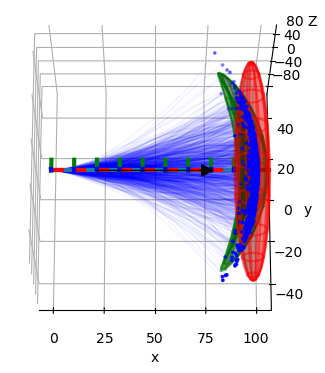
\includegraphics[width=0.4\textwidth]{images/state_estimation}\end{center}
\vskip -0.4cm
The \textbf{banana distribution} is Gaussian in exponential coordinates:
\[
\boldsymbol{T} = Exp(\mathcal{S}\theta) \overline{\boldsymbol{T}},\quad \textrm{with} \quad \mathcal{S}\theta \sim \mathcal{N}\left(\boldsymbol{0}, \boldsymbol{\Sigma}_{6 \times 6}\right)
\]
\end{frame}

\begin{frame}[fragile]{Concatenation of Uncertain Transforms}
\begin{lstlisting}[language=Python]
import pytransform3d.uncertainty as pu
# estimated mean pose (transformation matrix)
T_est = ...
# covariance in exponential coordinates
cov_est = ...
# mean offset (transformation matrix)
T_vel = ...
# covariance in exponential coordinates
cov_vel = ...

T_est, cov_est = pu.concat_globally_uncertain_transforms(
        T_est, cov_est,
        T_vel, cov_vel)
\end{lstlisting}
\end{frame}

\begin{frame}[fragile]{Transfer of Motions to Robotic Hand}
\begin{columns}
\begin{column}{0.4\textwidth}
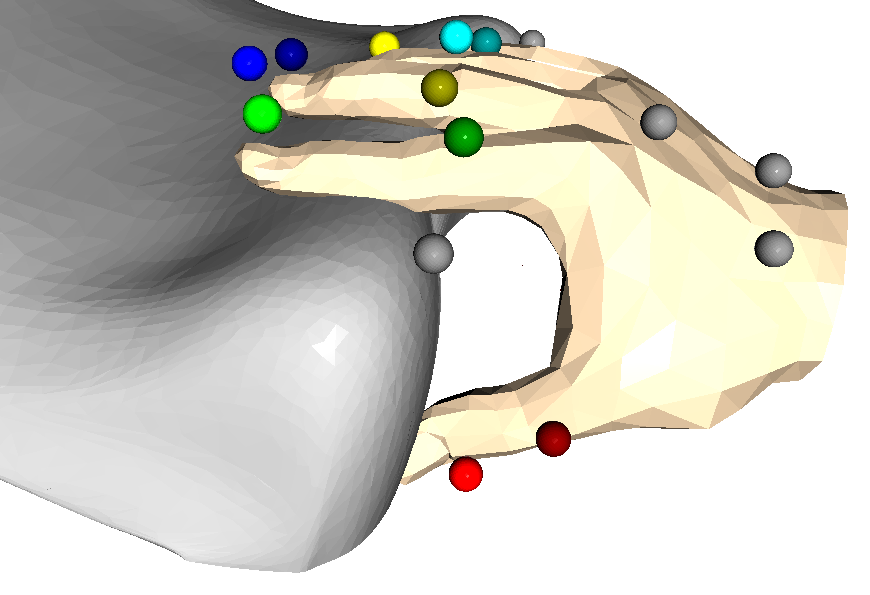
\includegraphics[width=\textwidth]{images/embodiment_record}
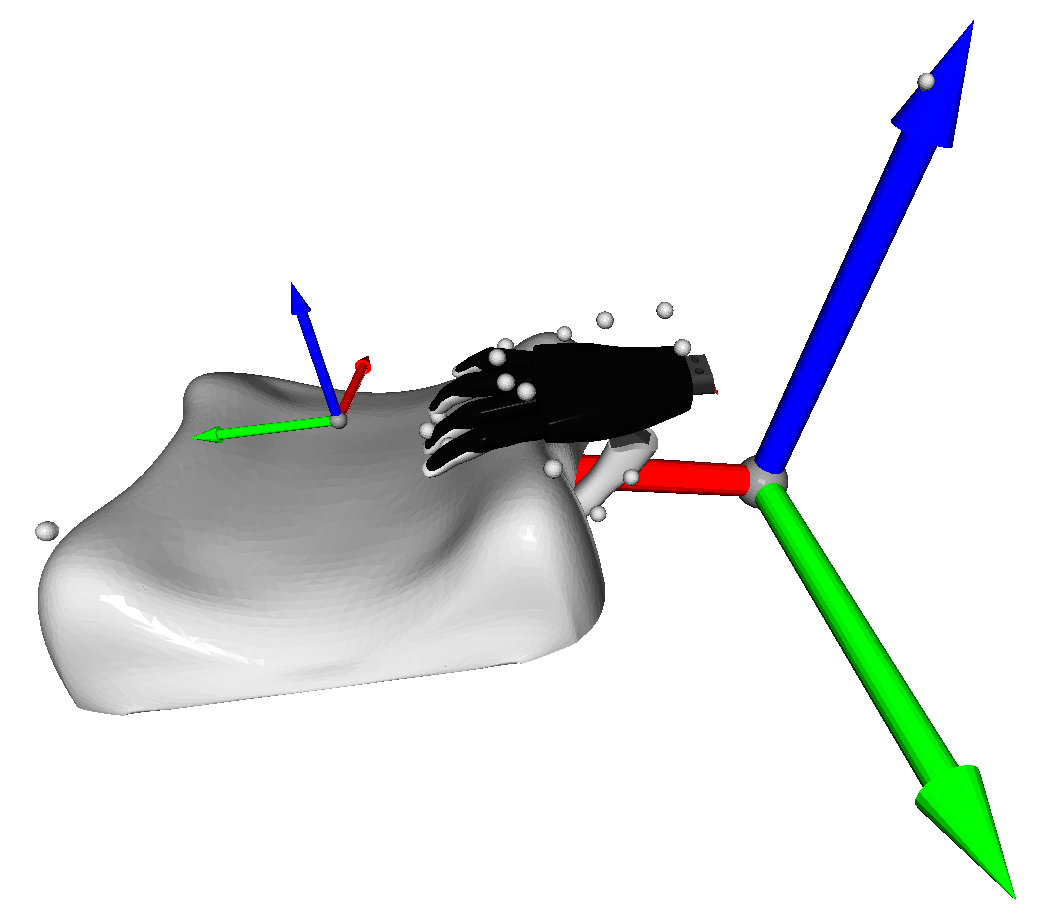
\includegraphics[width=\textwidth]{images/embodiment_mia}
\end{column}
\begin{column}{0.6\textwidth}
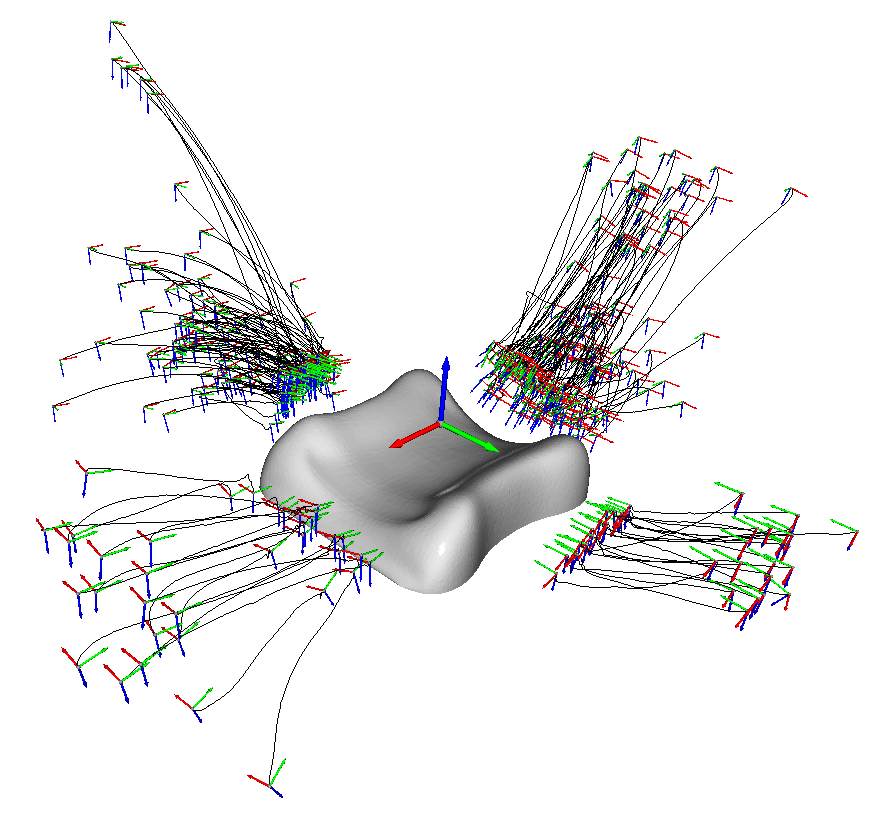
\includegraphics[width=\textwidth]{images/embodiment_dataset}
\end{column}
\end{columns}
{\small \url{https://github.com/dfki-ric/hand_embodiment}}
\end{frame}

\begin{frame}[plain,fragile]{Modeling Transformations}
\textbf{Mathematical notation:}
$\boldsymbol{T}_{BA}$ for transformation \textit{from frame} \texttt{A} \textit{to frame}
\texttt{B}. In concatenation, read from right to left:

\[
\boldsymbol{T}_{CB} \boldsymbol{T}_{BA} = \boldsymbol{T}_{C\cancel{B}} \boldsymbol{T}_{\cancel{B}A} = \boldsymbol{T}_{CA}.
\]

\vfill

\textbf{In code} we should prefer the notation \texttt{A2B}
for a transformation \textit{from frame} \texttt{A} \textit{to frame} \texttt{B}:

\begin{lstlisting}[language=Python]
from pytransform3d.transformations import concat
A2B = ...  # transformation from frame A to frame B
B2C = ...  # transformation from frame B to frame C
A2C = concat(A2B, B2C)
\end{lstlisting}
\end{frame}

\begin{frame}[plain,fragile]{Graphs of Transformations}
\begin{columns}
\begin{column}{0.4\textwidth}
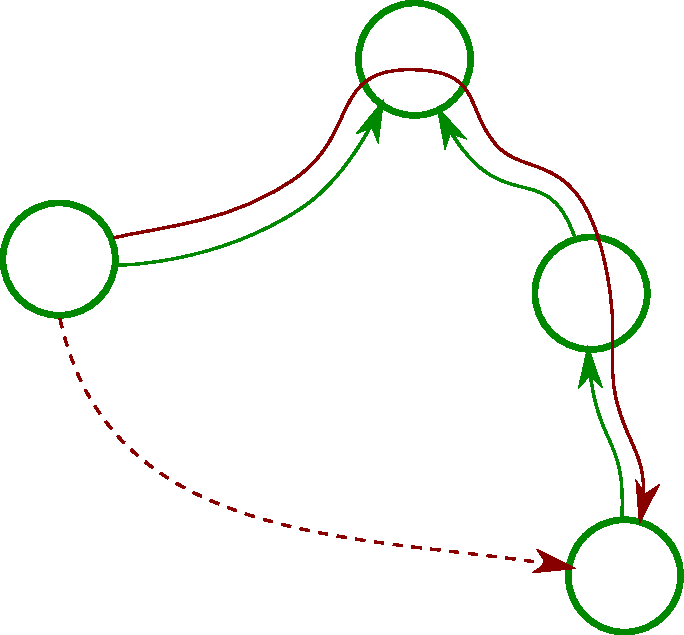
\includegraphics[width=\textwidth]{images/transform_graph}
\end{column}
\begin{column}{0.6\textwidth}
\begin{lstlisting}[language=Python]
from pytransform3d.transform_manager import TransformManager


tm = TransformManager()
tm.add_transform(
    "end-effector", "robot", ee2robot)
tm.add_transform(
    "camera", "robot", cam2robot)
tm.add_transform(
    "object", "camera", object2cam)

ee2object = tm.get_transform(
    "end-effector", "object")
\end{lstlisting}
\end{column}
\end{columns}

Examples: kinematic structures of robots (and other articulated bodies),
sequences of states, trajectories
\end{frame}

\begin{frame}[fragile]{Robot Kinematics}
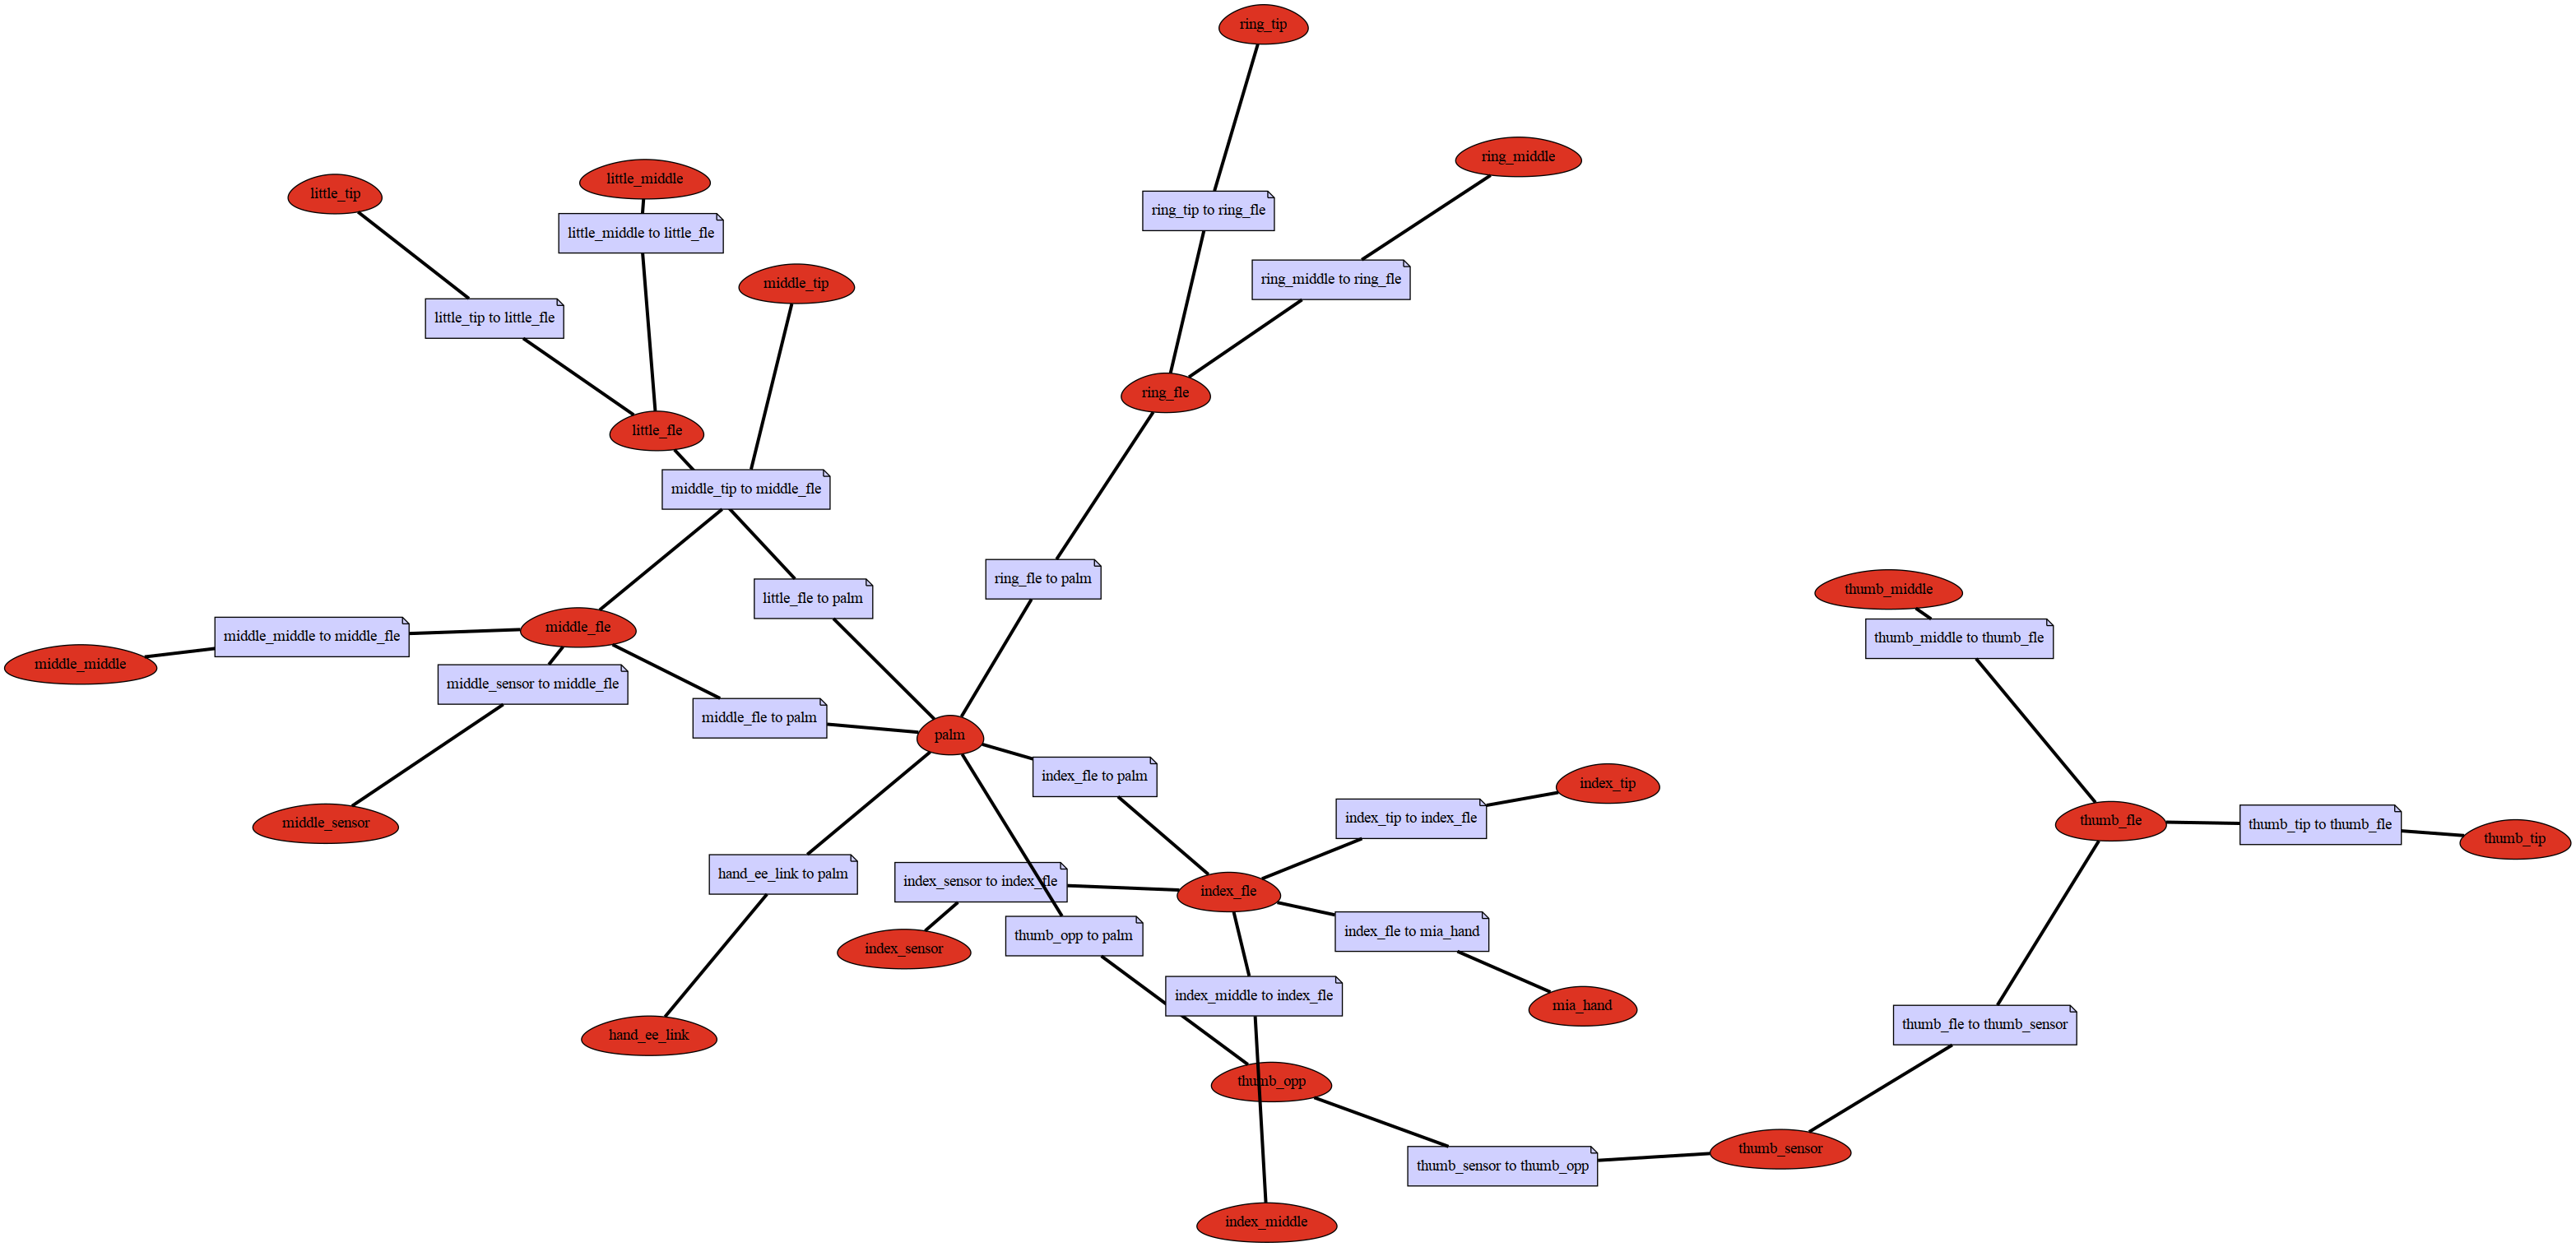
\includegraphics[width=\textwidth]{images/embodiment_graph}
\begin{lstlisting}[language=Python]
from pytransform3d.urdf import UrdfTransformManager
tm = UrdfTransformManager()
with open("robot.urdf", "r") as f:
    robot_urdf = f.read()
tm.load_urdf(robot_urdf)
tm.write_png(graph_filename)
\end{lstlisting}
\end{frame}

\begin{frame}{Collision Detection}
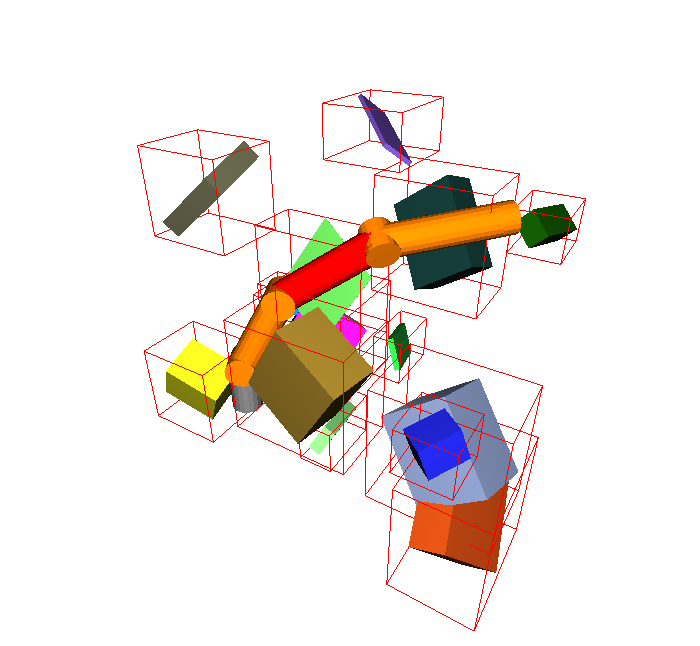
\includegraphics[width=0.7\textwidth]{images/collision_detection}
\end{frame}

\begin{frame}[fragile]{Collision Detection}
\begin{lstlisting}[language=Python]
from pytransform3d.urdf import UrdfTransformManager
from distance3d import broad_phase


# Load graph of transformations
robot_tree = UrdfTransformManager()
with open(filename, "r") as f:
    robot_urdf = f.read()
robot_tree.load_urdf(robot_urdf)

# Define configuration of robot
for joint_name in ["joint%d" % i for i in range(1, 7)]:
    robot_tree.set_joint(joint_name, 0.7)

# Construct bounding volume hierarchy for broad phase
robot_bvh = broad_phase.BoundingVolumeHierarchy(
    robot_tree, "robot_arm")
robot_bvh.fill_tree_with_colliders(robot_tree)
\end{lstlisting}
{\footnotesize Library: \url{https://github.com/AlexanderFabisch/distance3d}}
\end{frame}

\end{document}
